\documentclass{article}
\usepackage{amsmath,amssymb}
\usepackage{xcolor}
\usepackage[colorinlistoftodos]{todonotes}
\usepackage{tikz}
\usetikzlibrary{shapes.geometric,arrows.meta}
\usepackage[most]{tcolorbox}

\begin{document}

        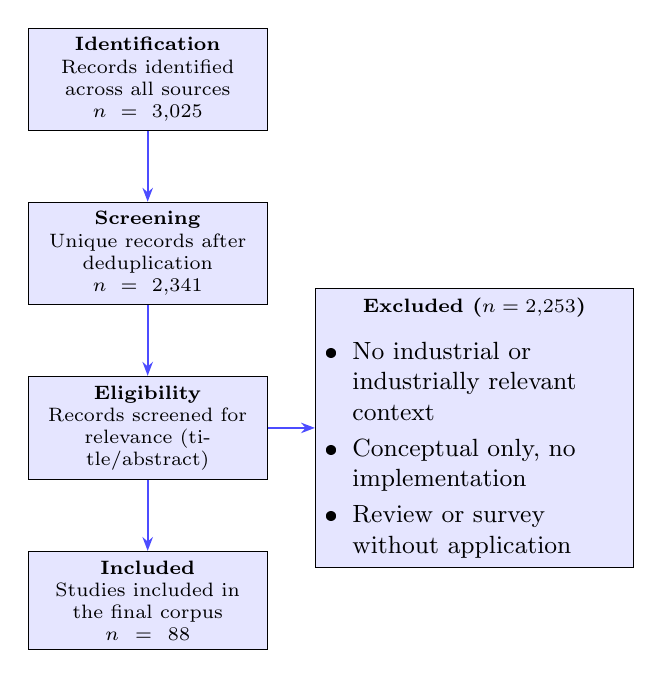
\begin{tikzpicture}[
    node distance=0.9cm and 0.6cm,
    box/.style={rectangle, draw, fill=blue!10, text width=2.8cm,
                text centered, minimum height=1.1cm,
                font=\scriptsize},
    reason/.style={rectangle, draw, fill=blue!10, text width=3.8cm,
                   text badly centered, minimum height=1.1cm,
                   font=\scriptsize},
    arrow/.style={-{Stealth[length=5pt]}, thick, blue!70},
    label/.style={font=\scriptsize, text=blue!70, fill=white, inner sep=1pt}
]

% Main flow (left column)
\node[box] (identify)
    {\textbf{Identification}\\Records identified\\across all sources\\$n = 3{,}025$};

\node[box, below=of identify] (screen)
    {\textbf{Screening}\\Unique records after\\deduplication\\$n = 2{,}341$};

\node[box, below=of screen] (eligible)
    {\textbf{Eligibility}\\Records screened for\\relevance (title/abstract)};

\node[box, below=of eligible] (include)
    {\textbf{Included}\\Studies included in\\the final corpus\\$n = 88$};

% Exclusion reason box (right column)
\node[reason, right=of eligible] (reason1) {%
    \textbf{Excluded ($n = 2{,}253$)}\\[3pt]
    {\small\setlength{\leftmargini}{10pt}%
    \raggedright
    \begin{itemize}\setlength\itemsep{0pt}\setlength\parsep{0pt}
      \item No industrial or industrially relevant context
      \item Conceptual only, no implementation
      \item Review or survey without application
    \end{itemize}}};

% Main vertical arrows
\draw[arrow] (identify) -- (screen);
\draw[arrow] (screen)   -- (eligible);
\draw[arrow] (eligible) -- (include);

% Exclusion arrow (horizontal, no label)
\draw[arrow] (eligible.east) -- (reason1.west);

\end{tikzpicture}

\end{document}